%!TEX root=../document.tex

\section{Grundanforderungen}
\label{sec:Ergebnisse}

\subsection{Installation Jenkins}

Der erste Punkt verlangt nach der Installation von Jenkins. Dafür wird die Software über die im Kurs abgelegte Verlinkung zu \textbf{https://jenkins.io/index.html} heruntergeladen. Nach der erfolgreichen installation sollte es möglich sein über den Browser auf \textbf{localhost:8080} Zugriff zu Jenkins zu bekommen. 

zunächst wurde ein neuer Benutzer mit Administrator-Rechten hinzugefügt. 
Dieser kann dann im /user/ - Tab eingesehen werden. 

\begin{figure}[!h]
	\begin{center}
		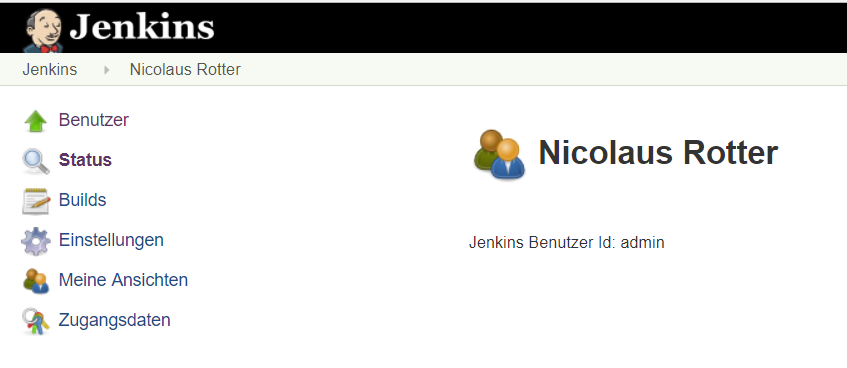
\includegraphics[width=0.7\textwidth]{images/userPNG.PNG}
	\end{center}
\end{figure}

\subsection{Installation Violations, Corbertura}

Zunächst wird die Installation der von uns benötigten Jenkins PlugIns verlangt. Dazu muss man auf \textbf{Jenkins verwalten -> PulgIns verwalten} gehen und im \textbf{Verfügbar}-Tab diese installieren. 

Falls dieser Schritt erfolgreich war sollten die PuligIns nach dem Neustart von Jenkins im \textbf{Installiert}-Tab erscheinen.

\subsection{Installation Nose, Coverage, Pylint}

Nun müssen folgende Packages über pip installiert werden:
\begin{itemize}
	\item Nose
	\item Coverage
	\item Pylint
\end{itemize}

\clearpage

Dies wurde im meinem Fall schon gemacht, daher bekomme ich folgende Rückmeldung in der Konsole:

\begin{figure}[!h]
	\begin{center}
		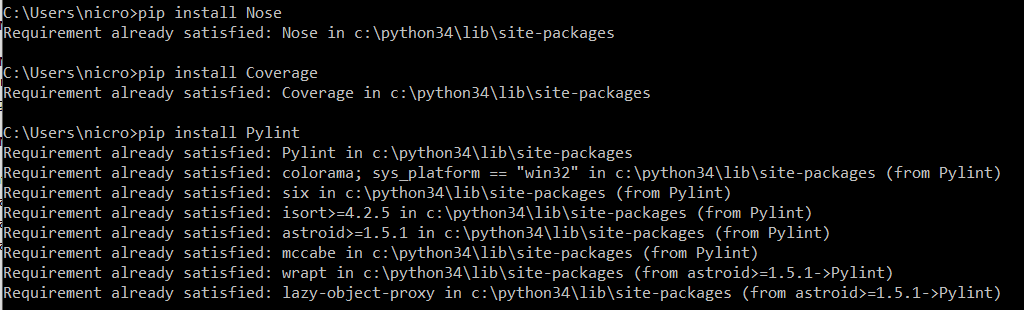
\includegraphics[width=0.7\textwidth]{images/pip.PNG}
	\end{center}
\end{figure}

